% Options for packages loaded elsewhere
\PassOptionsToPackage{unicode}{hyperref}
\PassOptionsToPackage{hyphens}{url}
%
\documentclass[
]{article}
\usepackage[top=2.5cm, bottom=2.5cm, left=2.8cm, right=2.8cm]{geometry}
\usepackage{amsmath,amssymb}
\usepackage{iftex}
\ifPDFTeX
  \usepackage[T1]{fontenc}
  \usepackage[utf8]{inputenc}
  \usepackage{textcomp}
\else
  \usepackage{unicode-math}
  \defaultfontfeatures{Scale=MatchLowercase}
  \defaultfontfeatures[\rmfamily]{Ligatures=TeX,Scale=1}
\fi
\usepackage{lmodern}
\usepackage{fancyhdr}
\pagestyle{fancy}
\fancyhf{}
\fancyhead[R]{\small\thepage}
\renewcommand{\headrulewidth}{0.4pt}
\fancypagestyle{plain}{\fancyhf{}\fancyhead[R]{\small\thepage}}
\ifPDFTeX\else
\fi
\IfFileExists{upquote.sty}{\usepackage{upquote}}{}
\IfFileExists{microtype.sty}{%
  \usepackage[]{microtype}
  \UseMicrotypeSet[protrusion]{basicmath}
}{}
\makeatletter
\@ifundefined{KOMAClassName}{%
  \IfFileExists{parskip.sty}{%
    \usepackage{parskip}
  }{%
    \setlength{\parindent}{0pt}
    \setlength{\parskip}{6pt plus 2pt minus 1pt}}
}{%
  \KOMAoptions{parskip=half}}
\makeatother
\usepackage{xcolor}
\usepackage{longtable,booktabs,array}
\usepackage{calc}
\usepackage{etoolbox}
\makeatletter
\patchcmd\longtable{\par}{\if@noskipsec\mbox{}\fi\par}{}{}
\makeatother
\IfFileExists{footnotehyper.sty}{\usepackage{footnotehyper}}{\usepackage{footnote}}
\makesavenoteenv{longtable}
\usepackage{graphicx}
\makeatletter
\def\maxwidth{\ifdim\Gin@nat@width>\linewidth\linewidth\else\Gin@nat@width\fi}
\def\maxheight{\ifdim\Gin@nat@height>\textheight\textheight\else\Gin@nat@height\fi}
\makeatother
\setkeys{Gin}{width=\maxwidth,height=\maxheight,keepaspectratio}
\makeatletter
\def\fps@figure{htbp}
\makeatother
\setlength{\emergencystretch}{3em}
\providecommand{\tightlist}{%
  \setlength{\itemsep}{0pt}\setlength{\parskip}{0pt}}
\setcounter{secnumdepth}{3}
\ifLuaTeX
  \usepackage{selnolig}
\fi
\usepackage{bookmark}
\IfFileExists{xurl.sty}{\usepackage{xurl}}{}
\urlstyle{same}
\hypersetup{
  pdftitle={Architekturdokumentation -- eBay-Klon als Microservices-Architektur},
  hidelinks,
  pdfcreator={LaTeX via pandoc}}
\usepackage{tikz}
\usetikzlibrary{shapes.geometric, shapes, arrows, positioning}
\usepackage[export]{adjustbox}
\usepackage{xparse}

% Deutsche Bezeichnungen für Inhaltsverzeichnis, Abbildungen und Tabellen
\renewcommand{\contentsname}{Inhaltsverzeichnis}
\renewcommand{\listfigurename}{Abbildungsverzeichnis}
\renewcommand{\listtablename}{Tabellenverzeichnis}
\renewcommand{\figurename}{Abbildung}
\renewcommand{\tablename}{Tabelle}

\usepackage{tabularx}
\usepackage{booktabs}
\usepackage[table]{xcolor}
\usepackage{float}
\colorlet{tableHeaderColor}{gray!25}
\colorlet{tableRowColor}{gray!14}


\newcommand{\includegraphicsifexists}[2]{%
  \IfFileExists{#1}{%
    \includegraphics[width=\textwidth,height=#2,keepaspectratio]{#1}%
  }{%
    \fbox{\parbox{\dimexpr\textwidth-2\fboxsep-2\fboxrule\relax}{\centering\vspace{2cm}
      \textbf{Bild nicht gefunden}\\[4pt]
      \texttt{#1}\\[4pt]
      Aus \texttt{.drawio} als PNG exportieren und in \texttt{images/} ablegen\vspace{2cm}}}%
  }%
}


\begin{document}
\begin{titlepage}
\centering
\vspace*{\fill}
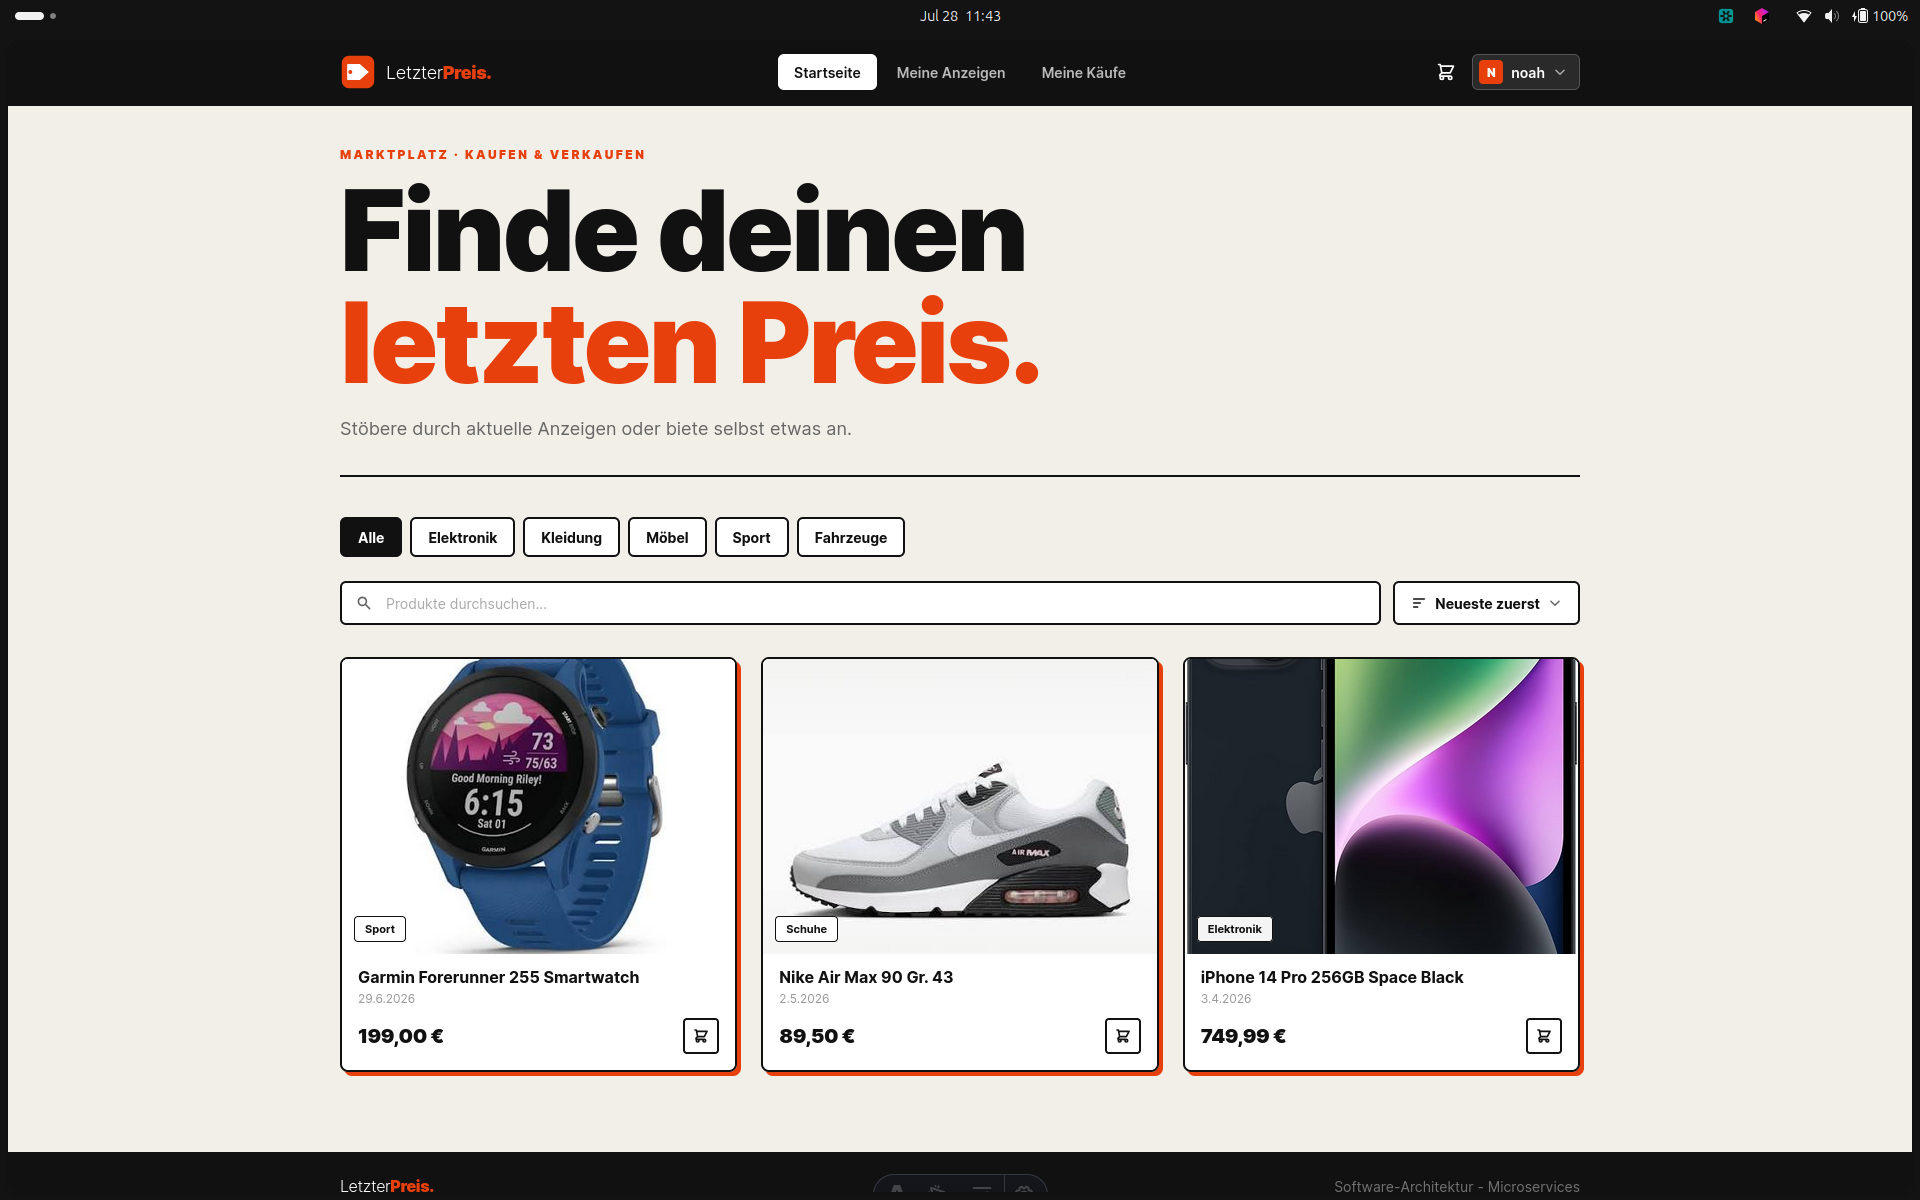
\includegraphics[width=0.95\textwidth]{images/front_page.png}\\[12pt]
{\Huge Architekturdokumentation}\\[4pt]
{\Large eBay-Klon als Microservices-Architektur}\\[24pt]
{\large Gruppe 5 -- Software-Architektur}\\[8pt]
Dominik Duken 21947166\\
Noah Preyer 35797\\
Ilker Türk 29963\\[8pt]
Juli 2026
\vspace*{\fill}
\end{titlepage}
\clearpage
\author{Ilker Türk}
\tableofcontents
\newpage

\section{Einführung und Ziele}

\subsection{Aufgabenstellung}

Die Aufgabenstellung bestand darin, einen Architekturstil anhand einer
Beispielanwendung umzusetzen.
Dabei fiel die Wahl auf die Microservice-Architektur.

Als Beispielanwendung dient eine E-Commerce-Plattform,
deren Funktionen sich gut in fachlich getrennte Bereiche aufteilen lassen.
Der vollständige Quellcode ist im zugehörigen GitHub-Repository verfügbar:

\begin{center}
    \url{https://github.com/noah-preyer/SS26_Software_Architektur_Ebay2.git}
\end{center}

Die Umsetzung konzentriert sich auf die folgenden Kernfunktionen:

\subsection{Kernfunktionen}

\begin{itemize}
\item Registrierung und Anmeldung mittels JWT
\item Erstellen, Bearbeiten, Löschen und Suchen von Produkten
\item beispielhafte Kaufabwicklung und E-Mail-Benachrichtigungen
\end{itemize}


\subsection{Qualitätsziele}

\begin{table}[ht]
    \centering
    {
        \renewcommand{\arraystretch}{1.5}
        \rowcolors{2}{tableRowColor}{white}

        \begin{tabularx}{\linewidth}{
                >{\bfseries\raggedright\arraybackslash}p{0.20\linewidth}
                >{\raggedright\arraybackslash}X
        }
        \toprule
        Qualitätsziel & Beschreibung \\
        \midrule

        Modularität &
        Die Services sollen fachlich klar voneinander abgegrenzt sein. \\

        Sicherheit &
        Geschützte Service-Funktionen sollen nur für berechtigte Benutzer zugänglich sein. \\

        Erweiterbarkeit &
        Neue Services sollen mit möglichst wenigen Änderungen am bestehenden System ergänzt werden können. \\

        Skalierbarkeit &
        Ein Service soll bei Bedarf unabhängig vom restlichen System durch mehrere Replikate skaliert werden können. \\

        Fehlertoleranz &
        Der Ausfall eines Services soll andere Bereiche möglichst nicht
        beeinträchtigen. \\

        \bottomrule
        \end{tabularx}
    }

    \caption{Qualitätsziele der Architektur}
    \label{tab:qualitaetsziele}
\end{table}
\section{Randbedingungen}

Der Schwerpunkt des Projekts liegt auf der Umsetzung und Bewertung der Microservice-Architektur.
Der Funktionsumfang der Beispielanwendung wurde daher bewusst auf wenige Kernfunktionen begrenzt.

Für die Auswahl der Programmiersprachen, Frameworks und Werkzeuge bestanden
keine festen Vorgaben.
\section{Kontextabgrenzung}

\subsection{Fachlicher Kontext}

Die E-Commerce-Plattform wird von registrierten und nicht registrierten Benutzern verwendet.
Nicht registrierte Benutzer können Produkte suchen und anzeigen sowie ein Benutzerkonto erstellen.
Registrierte Benutzer können zusätzlich Produkte einstellen und kaufen.

Nach einem erfolgreichen Kauf wird eine Bestellbestätigung über einen externen E-Mail-Dienst versendet.


\subsection{Technischer Kontext}

Das System tritt nach außen als eine zusammenhängende Anwendung auf und wird über einen Webbrowser genutzt.
Das Frontend kommuniziert über HTTP/REST mit dem API Gateway, das den zentralen Einstiegspunkt bildet.

Die interne Kommunikation zwischen den Services erfolgt über REST und MQTT.
Die externen Schnittstellen sind in
Tabelle~\ref{tab:externe_schnittstellen} dargestellt.

\subsection{Externe Schnittstellen}

\begin{table}[ht]
    \centering
    {
        \renewcommand{\arraystretch}{1.5}
        \rowcolors{2}{tableRowColor}{white}


        \begin{tabularx}{\linewidth}{
                >{\bfseries\raggedright\arraybackslash}p{0.20\linewidth}
                >{\raggedright\arraybackslash}p{0.18\linewidth}
                >{\raggedright\arraybackslash}X
        }
        \toprule
        Gegenstelle & Richtung & Inhalt und Protokoll \\
        \midrule

        Webbrowser &
        Bidirektional &
        Bedienung der Plattform über HTTP/REST. \\

        SMTP-Server &
        Ausgehend &
        Versand von Bestellbestätigungen über SMTP mit STARTTLS
        auf Port 587. \\

        \bottomrule
        \end{tabularx}
    }

    \caption{Externe Schnittstellen}
    \label{tab:externe_schnittstellen}

\end{table}
\begin{figure}[H]
    \centering
    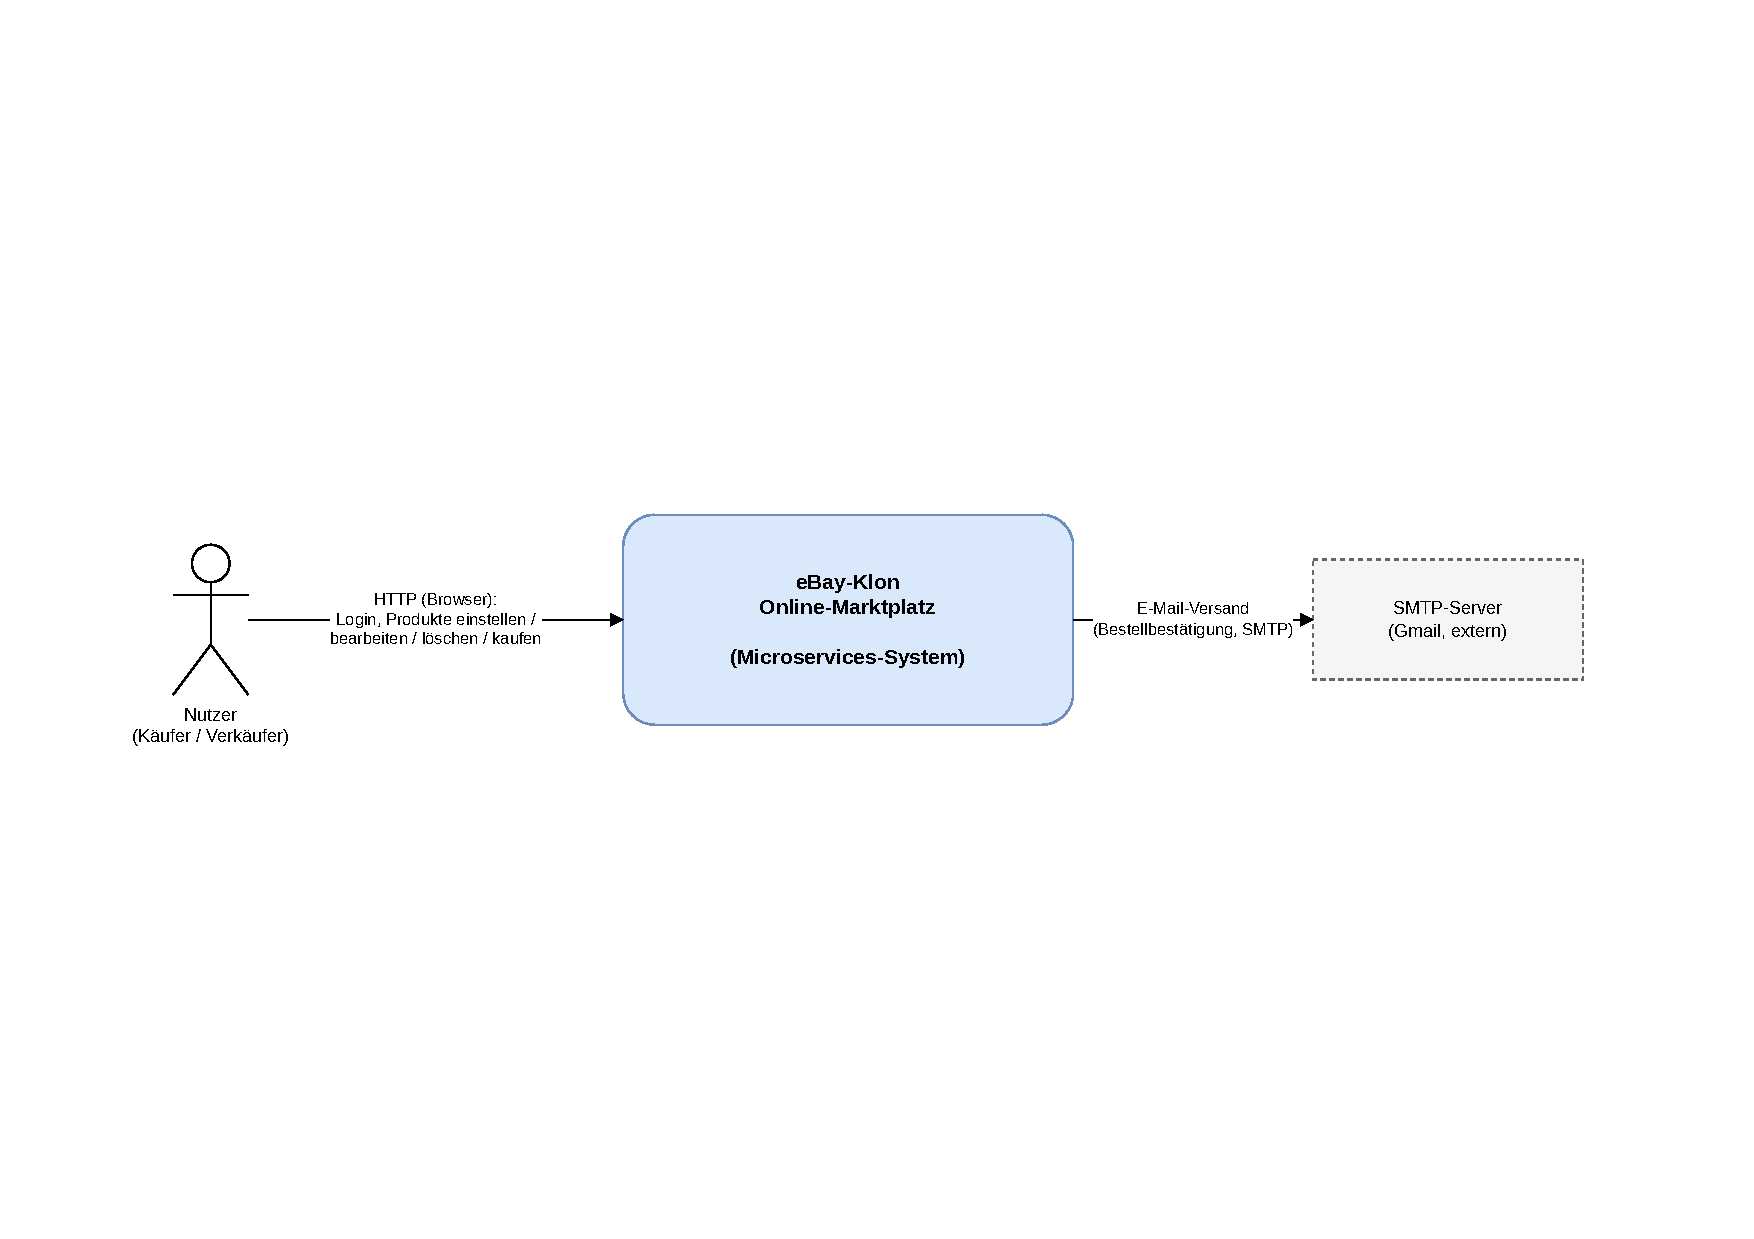
\includegraphics[width=\linewidth,trim=2cm 3cm 2cm 3cm,clip]{images/01-kontextdiagramm.pdf}
    \caption{Kontextdiagramm der E-Commerce-Plattform}
    \label{fig:kontextdiagramm}
\end{figure}
\section{Lösungsstrategie}

Die Anwendung wurde als Microservice-Architektur umgesetzt. Die wichtigsten
Lösungsansätze sind in Tabelle~\ref{tab:loesungsstrategie} zusammengefasst.

\begin{table}[ht]
    \centering

    {
        \renewcommand{\arraystretch}{1.5}
        \rowcolors{2}{tableRowColor}{white}

        \begin{tabularx}{\linewidth}{
                >{\bfseries\raggedright\arraybackslash}p{0.20\linewidth}
                >{\raggedright\arraybackslash}p{0.35\linewidth}
                >{\raggedright\arraybackslash}X
        }
        \toprule
        Bereich & Umsetzung & Begründung \\
        \midrule

        Systemaufteilung &
        Aufteilung in fachlich getrennte Microservices &
        Unterstützt Modularität und Erweiterbarkeit. \\

        Betrieb &
        Containerisierung mit Docker &
        Vereinfacht die Bereitstellung und lokale Ausführung der Anwendung. \\

        Zugriff &
        Zentrales API Gateway mit JWT-Validierung &
        Fasst die einzelnen Services nach außen zu einem einheitlichen System
        zusammen und stellt einen zentralen, geschützten Zugang bereit. \\

        Kommunikation &
        REST für Anfragen und MQTT für Ereignisse &
        Schafft klar definierte Kommunikationswege. \\

        Technologien &
        Spring Boot, Flask, Astro und SolidJS &
        Ermöglicht passende Technologien für jeden Bereich. \\

        \bottomrule
        \end{tabularx}
    }

    \caption{Zentrale Lösungsansätze}
    \label{tab:loesungsstrategie}
\end{table}
\section{Bausteinsicht}

\subsection{Ebene 1: Das Gesamtsystem}

Das System besteht aus sieben eigenständig ausgelieferten Bausteinen sowie
einem Nachrichtenbroker und einem Loadbalancer.
Die Aufteilung orientiert sich an den fachlichen Verantwortungsbereichen des Systems.
Abbildung~\ref{fig:bausteinsicht} zeigt den Aufbau des Systems.

\begin{figure}[H]
    \centering
    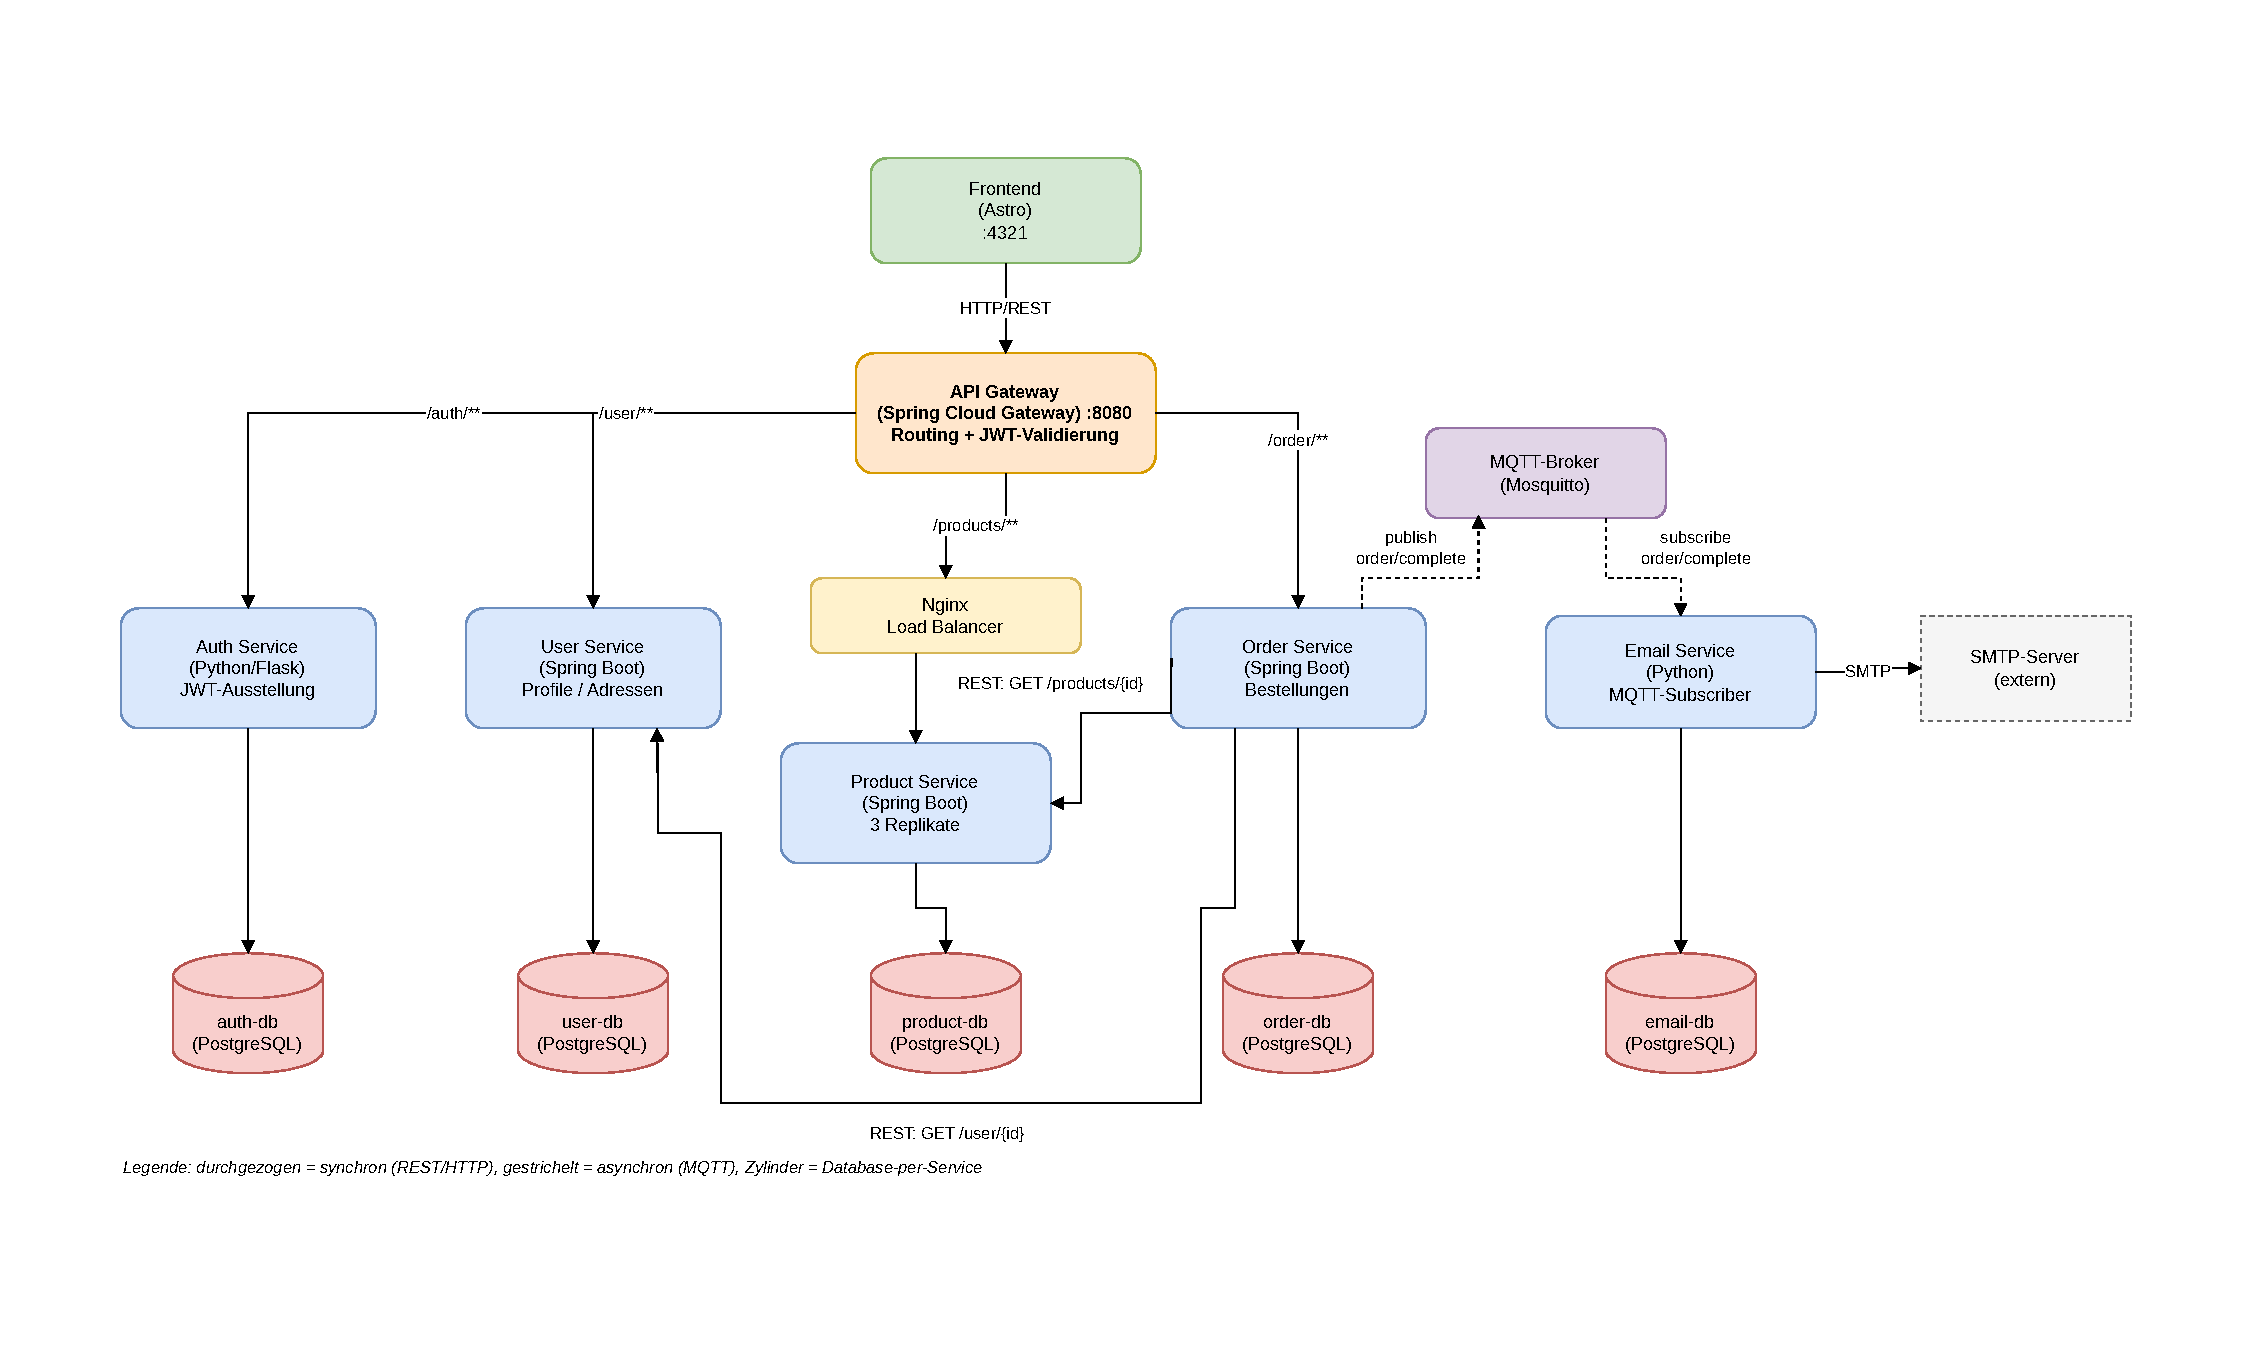
\includegraphics[width=\linewidth,trim=2cm 2cm 2cm 2cm,clip]{images/02-bausteinsicht}
    \caption{Bausteinsicht}
    \label{fig:bausteinsicht}
\end{figure}

Die Verantwortlichkeiten der einzelnen Bausteine sind in Tabelle~\ref{tab:bausteine} zusammengefasst.
    {
    \renewcommand{\arraystretch}{1.5}

    \begin{longtable}{@{}
            >{\bfseries\raggedright\arraybackslash}p{0.18\linewidth}
            >{\raggedright\arraybackslash}p{0.82\linewidth}
        @{}}
        \caption{Verantwortlichkeiten der Bausteine}
        \label{tab:bausteine} \\

        \toprule
        \rowcolor{tableHeaderColor}
        Baustein & Verantwortung \\
        \midrule
        \endfirsthead

        \multicolumn{2}{@{}l}{%
            \tablename\ \thetable{} -- Fortsetzung
        } \\

        \toprule
        \rowcolor{tableHeaderColor}
        Baustein & Verantwortung \\
        \midrule
        \endhead

        \midrule
        \multicolumn{2}{r@{}}{Fortsetzung auf der nächsten Seite} \\
        \endfoot

        \bottomrule
        \endlastfoot

        Frontend &
        Mit Astro und SolidJS umgesetzt. Stellt Komponenten und Seiten für
        Produkte, Warenkorb und Benutzerkonto bereit. \\

        \rowcolor{tableRowColor}
        API Gateway &
        Als Spring-Cloud-Gateway-Anwendung umgesetzt. Enthält die Routen zu den
        Services sowie einen Filter zur JWT-Validierung. \\

        Auth Service &
        Als Flask-Anwendung umgesetzt. Enthält REST-Endpunkte für Registrierung
        und Anmeldung sowie die Erzeugung von JWTs. \\

        \rowcolor{tableRowColor}
        User Service &
        Als Spring-Boot-Anwendung mit Controller-, Service- und
        Repository-Schicht umgesetzt. Verwaltet Benutzerprofile und
        Lieferadressen. \\

        Product Service &
        Als Spring-Boot-Anwendung mit Controller-, Service- und
        Repository-Schicht umgesetzt. Verwaltet Produkte und deren
        Verkaufsstatus. \\

        \rowcolor{tableRowColor}
        Order Service &
        Als Spring-Boot-Anwendung umgesetzt. Koordiniert den Kaufvorgang über
        REST-Clients, speichert Bestellungen und veröffentlicht
        Bestellereignisse über MQTT. \\

        Email Service &
        Als Python-Anwendung mit \texttt{paho-mqtt} umgesetzt. Abonniert
        Bestellereignisse, rendert E-Mail-Vorlagen und versendet
        Bestellbestätigungen. \\

        \rowcolor{tableRowColor}
        MQTT-Broker &
        Vermittelt die asynchronen Bestellereignisse zwischen Order Service
        und Email Service. \\

        Nginx &
        Verteilt Produktanfragen im Round-Robin-Verfahren auf die drei
        Instanzen des Product Service. \\

    \end{longtable}
}

\subsection{Ebene 2 -- Order Service (exemplarisch)}

Der Order Service ist intern in Controller, Geschäftslogik,
Datenzugriff und ausgehende Clients gegliedert.
Die ausgehenden REST- und MQTT-Aufrufe sind in eigenen Client-Klassen gekapselt.
Dadurch bleibt die eigentliche Kaufabwicklung im \texttt{OrderService} weitgehend unabhängig von den verwendeten Kommunikationsprotokollen.

Tabelle~\ref{tab:order-codebausteine} beschreibt die wichtigsten
Codebausteine und Abbildung~\ref{fig:order_service} zeigt deren
Abhängigkeiten.
\begin{table}[H]
    \centering
    \caption{Codebausteine des Order Service}
    \label{tab:order-codebausteine}

    \renewcommand{\arraystretch}{1.4}

    \begin{tabularx}{\linewidth}{@{}
            >{\bfseries\raggedright\arraybackslash}p{0.27\linewidth}
            >{\raggedright\arraybackslash}X
        @{}}

        \toprule
        \rowcolor{tableHeaderColor}
        Codebaustein & Aufgabe \\
        \midrule

        OrderController &
        Stellt die REST-Endpunkte des Order Service bereit, nimmt Anfragen
        entgegen und delegiert die Verarbeitung an den
        \texttt{OrderService}. \\

        \rowcolor{tableRowColor}
        OrderService &
        Enthält die Geschäftslogik des Kaufvorgangs. Prüft Produkte,
        reserviert Artikel, legt Bestellungen an und löst die
        Bestellbestätigung aus. \\

        OrderRepository &
        Kapselt mit Spring Data JPA den Zugriff auf die
        \texttt{order-service-db}. \\

        \rowcolor{tableRowColor}
        ProductServiceClient &
        Kapselt die REST-Aufrufe zum Product Service, beispielsweise zum
        Abrufen, Reservieren und Freigeben eines Produkts. \\

        UserServiceClient &
        Ruft die Benutzerdaten und die E-Mail-Adresse des Käufers beim
        User Service ab. \\

        \rowcolor{tableRowColor}
        EmailServiceClient &
        Veröffentlicht nach einem erfolgreichen Kauf ein MQTT-Ereignis auf
        dem Topic \texttt{order/complete}. \\

        OrderStatusScheduler &
        Sucht regelmäßig nach fälligen Bestellungen und führt die
        Statusübergänge \texttt{CREATED}, \texttt{PAID},
        \texttt{SHIPPED} und \texttt{DELIVERED} aus. \\

        \rowcolor{tableRowColor}
        GlobalExceptionHandler &
        Wandelt Exceptions in einheitliche HTTP-Fehlerantworten um. \\

        DTOs und Domänenklassen &
        Enthalten die internen Bestellobjekte sowie die Datenmodelle für die
        Kommunikation mit Product Service und User Service. \\

        \bottomrule
    \end{tabularx}
\end{table}

\begin{figure}[H]
    \centering
    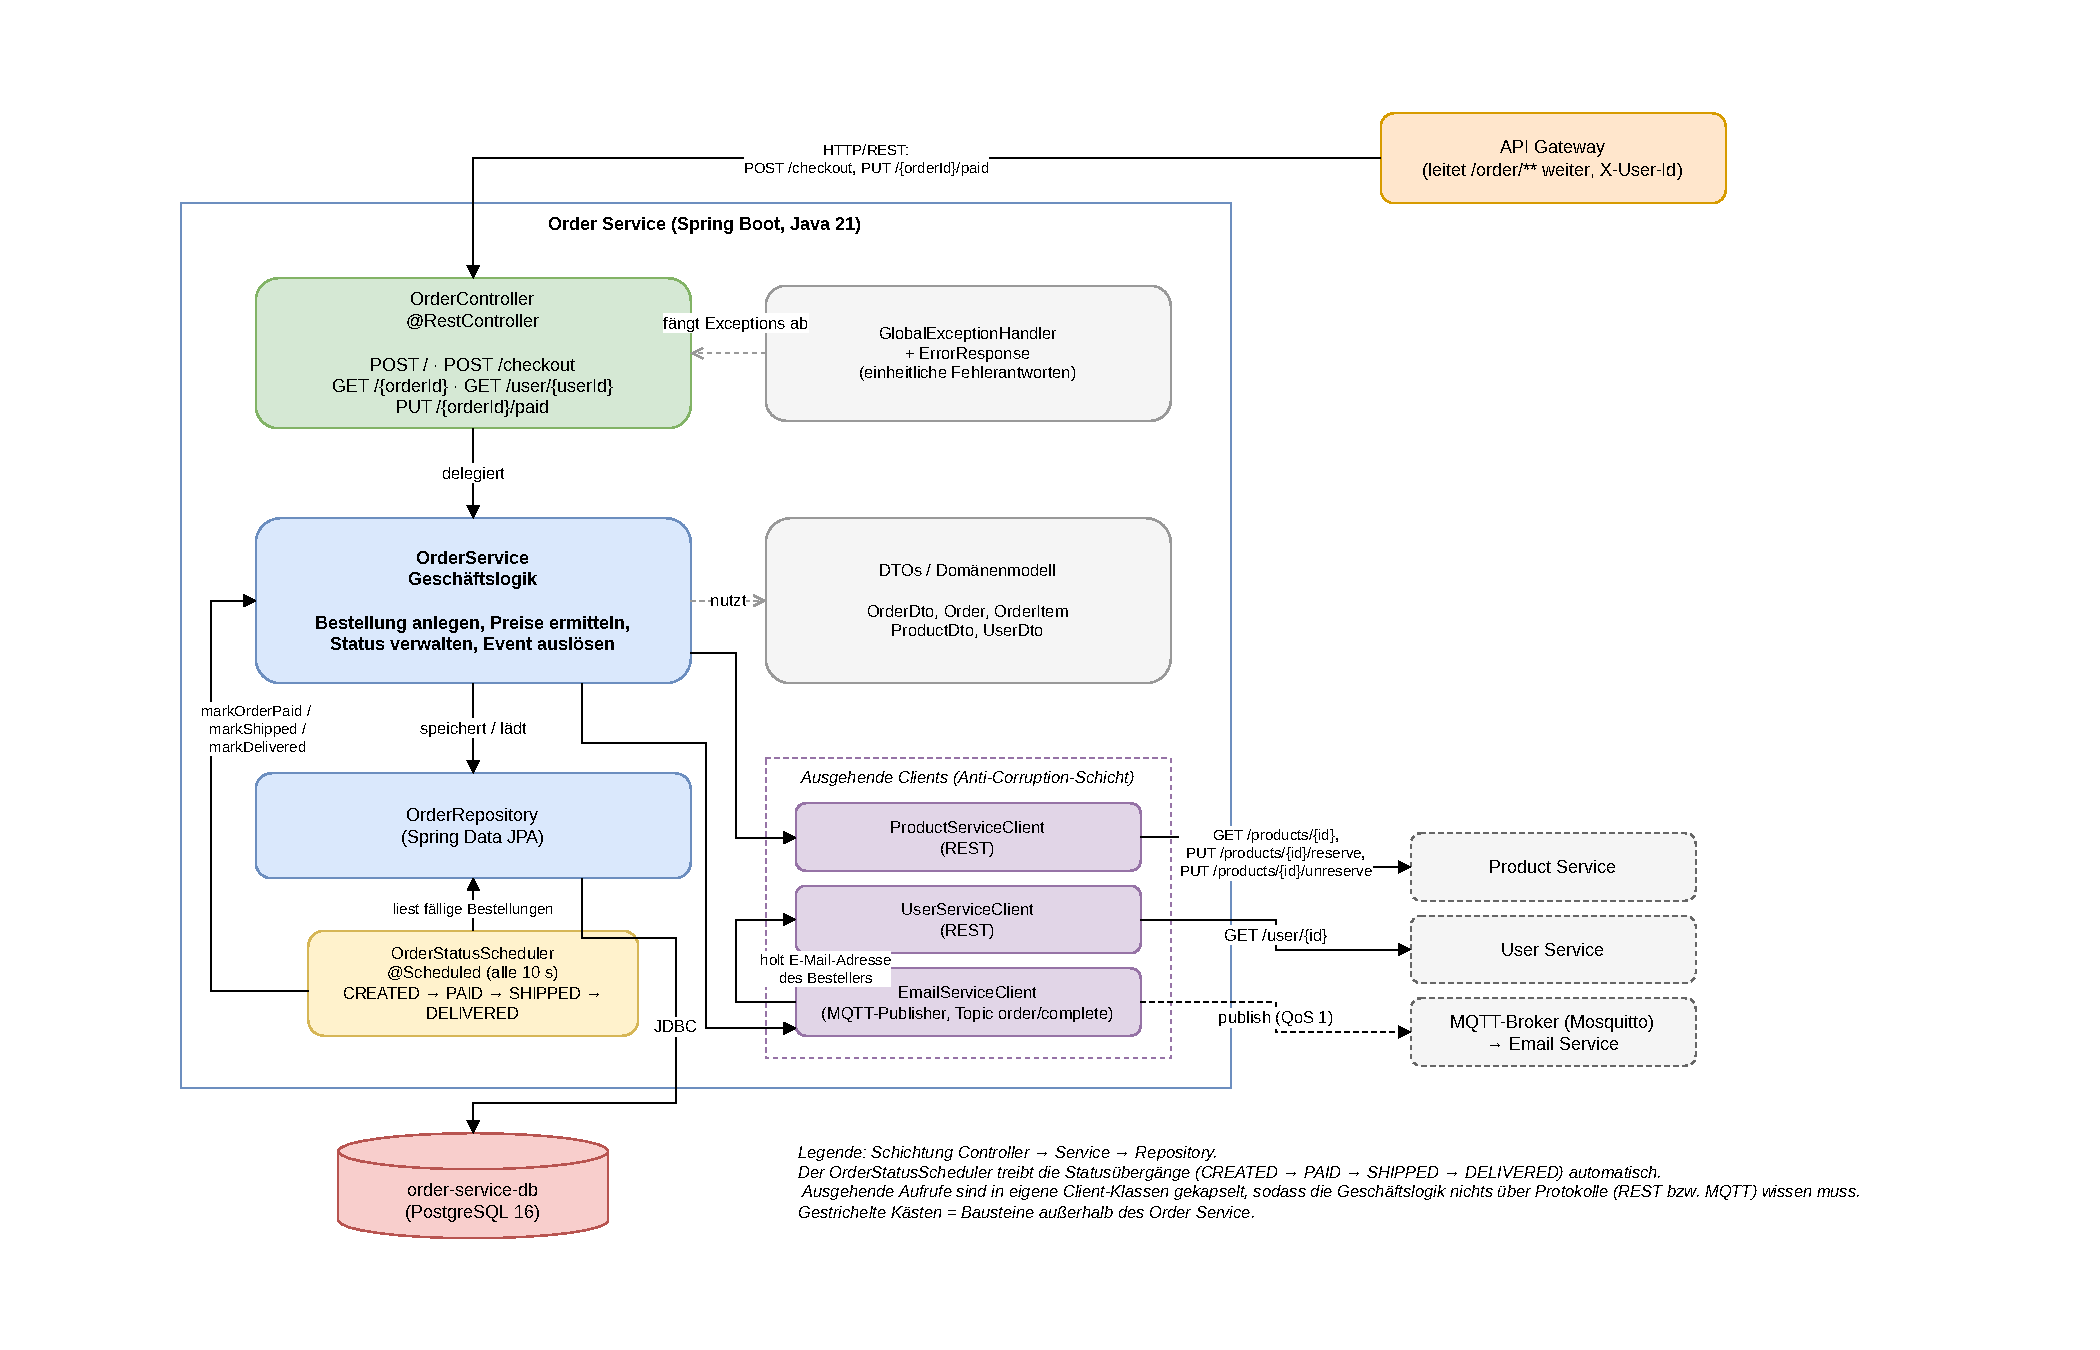
\includegraphics[width=\linewidth,trim=3cm 1cm 4cm 1cm,clip]{images/06-whitebox-order-service}
    \caption{Order Service}
    \label{fig:order_service}
\end{figure}

\section{Laufzeitsicht}

\subsection{Anmeldung und Zugriff auf geschützte Bereiche}

Bei der Anmeldung leitet das API Gateway die Zugangsdaten an den Auth Service weiter.
Nach erfolgreicher Prüfung stellt dieser ein 60 Minuten gültiges JWT aus.

Bei geschützten Aufrufen validiert das API Gateway das Token.
Ungültige oder abgelaufene Tokens werden mit \texttt{401 Unauthorized} abgewiesen.
Andernfalls wird die Benutzer-ID ausgelesen und an den zuständigen Service weitergegeben.
Der vollständige Ablauf ist in Abbildung~\ref{fig:login} dargestellt.

\begin{figure}[htbp]
    \centering
    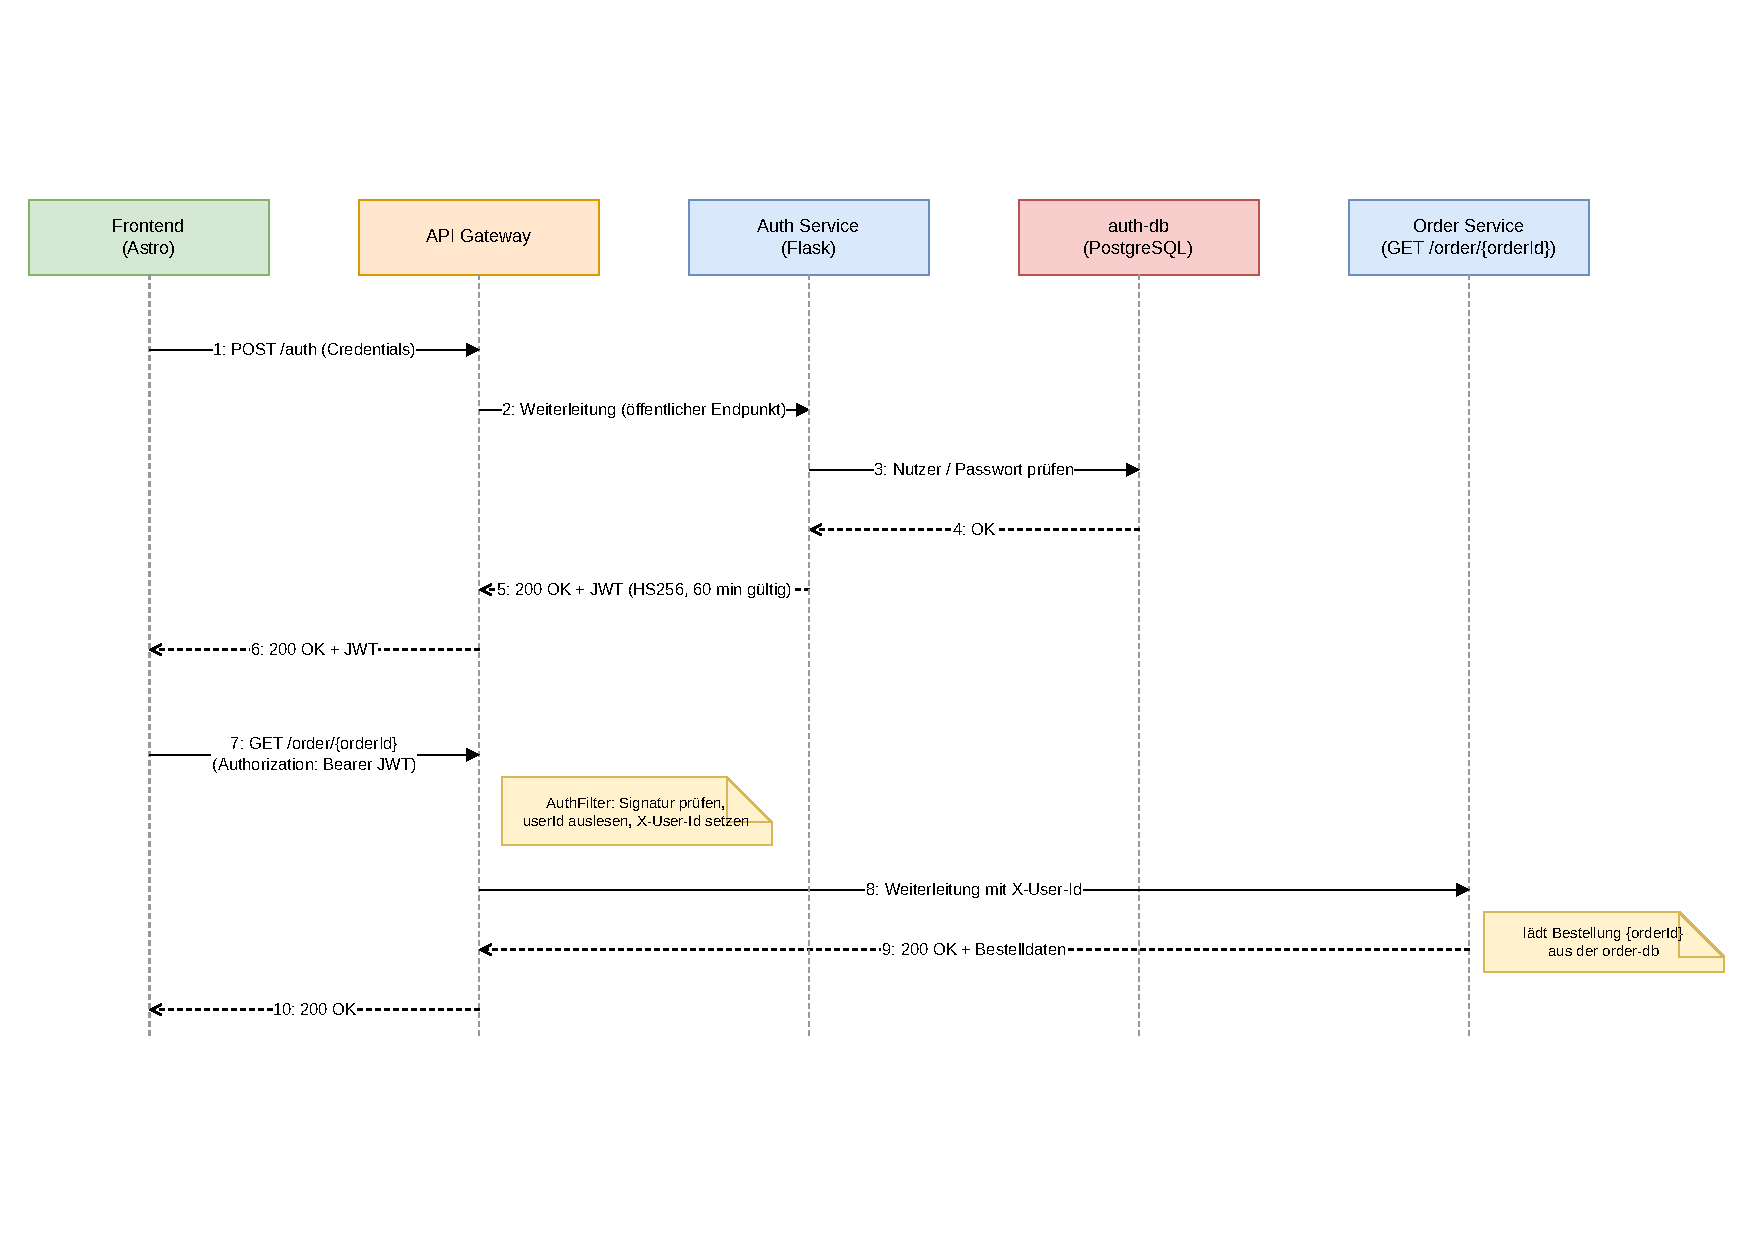
\includegraphics[width=\linewidth]{images/04-sequenz-login.pdf}
    \caption{Anmeldung und anschließender Zugriff mit Token}
    \label{fig:login}
\end{figure}

\subsection{Kauf von Artikeln}

Beim Kauf übermittelt das Frontend alle Artikel des Warenkorbs in einer Anfrage.
Der Order Service prüft beim Product Service,
ob die Artikel noch verfügbar sind und nicht dem Käufer selbst gehören.
Schlägt eine Prüfung fehl, wird der gesamte Kauf abgebrochen.

Anschließend markiert der Order Service die Artikel als verkauft.
Tritt dabei ein Fehler auf, werden bereits vorgenommene Änderungen zurückgesetzt.
Danach wird die Bestellung im Status \texttt{CREATED} gespeichert und die E-Mail-Adresse beim User Service abgerufen.

Der Order Service veröffentlicht über MQTT ein Ereignis,
das vom Email Service unabhängig verarbeitet wird.
Dadurch kann die Bestellbestätigung versendet werden,
ohne die Antwort an den Benutzer zu verzögern.

Die weiteren Statusübergänge von \texttt{CREATED} über \texttt{PAID} und
\texttt{SHIPPED} bis \texttt{DELIVERED} werden automatisch vom
Order Status Scheduler durchgeführt.
Der vollständige Ablauf ist in Abbildung~\ref{fig:buying} dargestellt.


\begin{figure}[htbp]
    \centering
    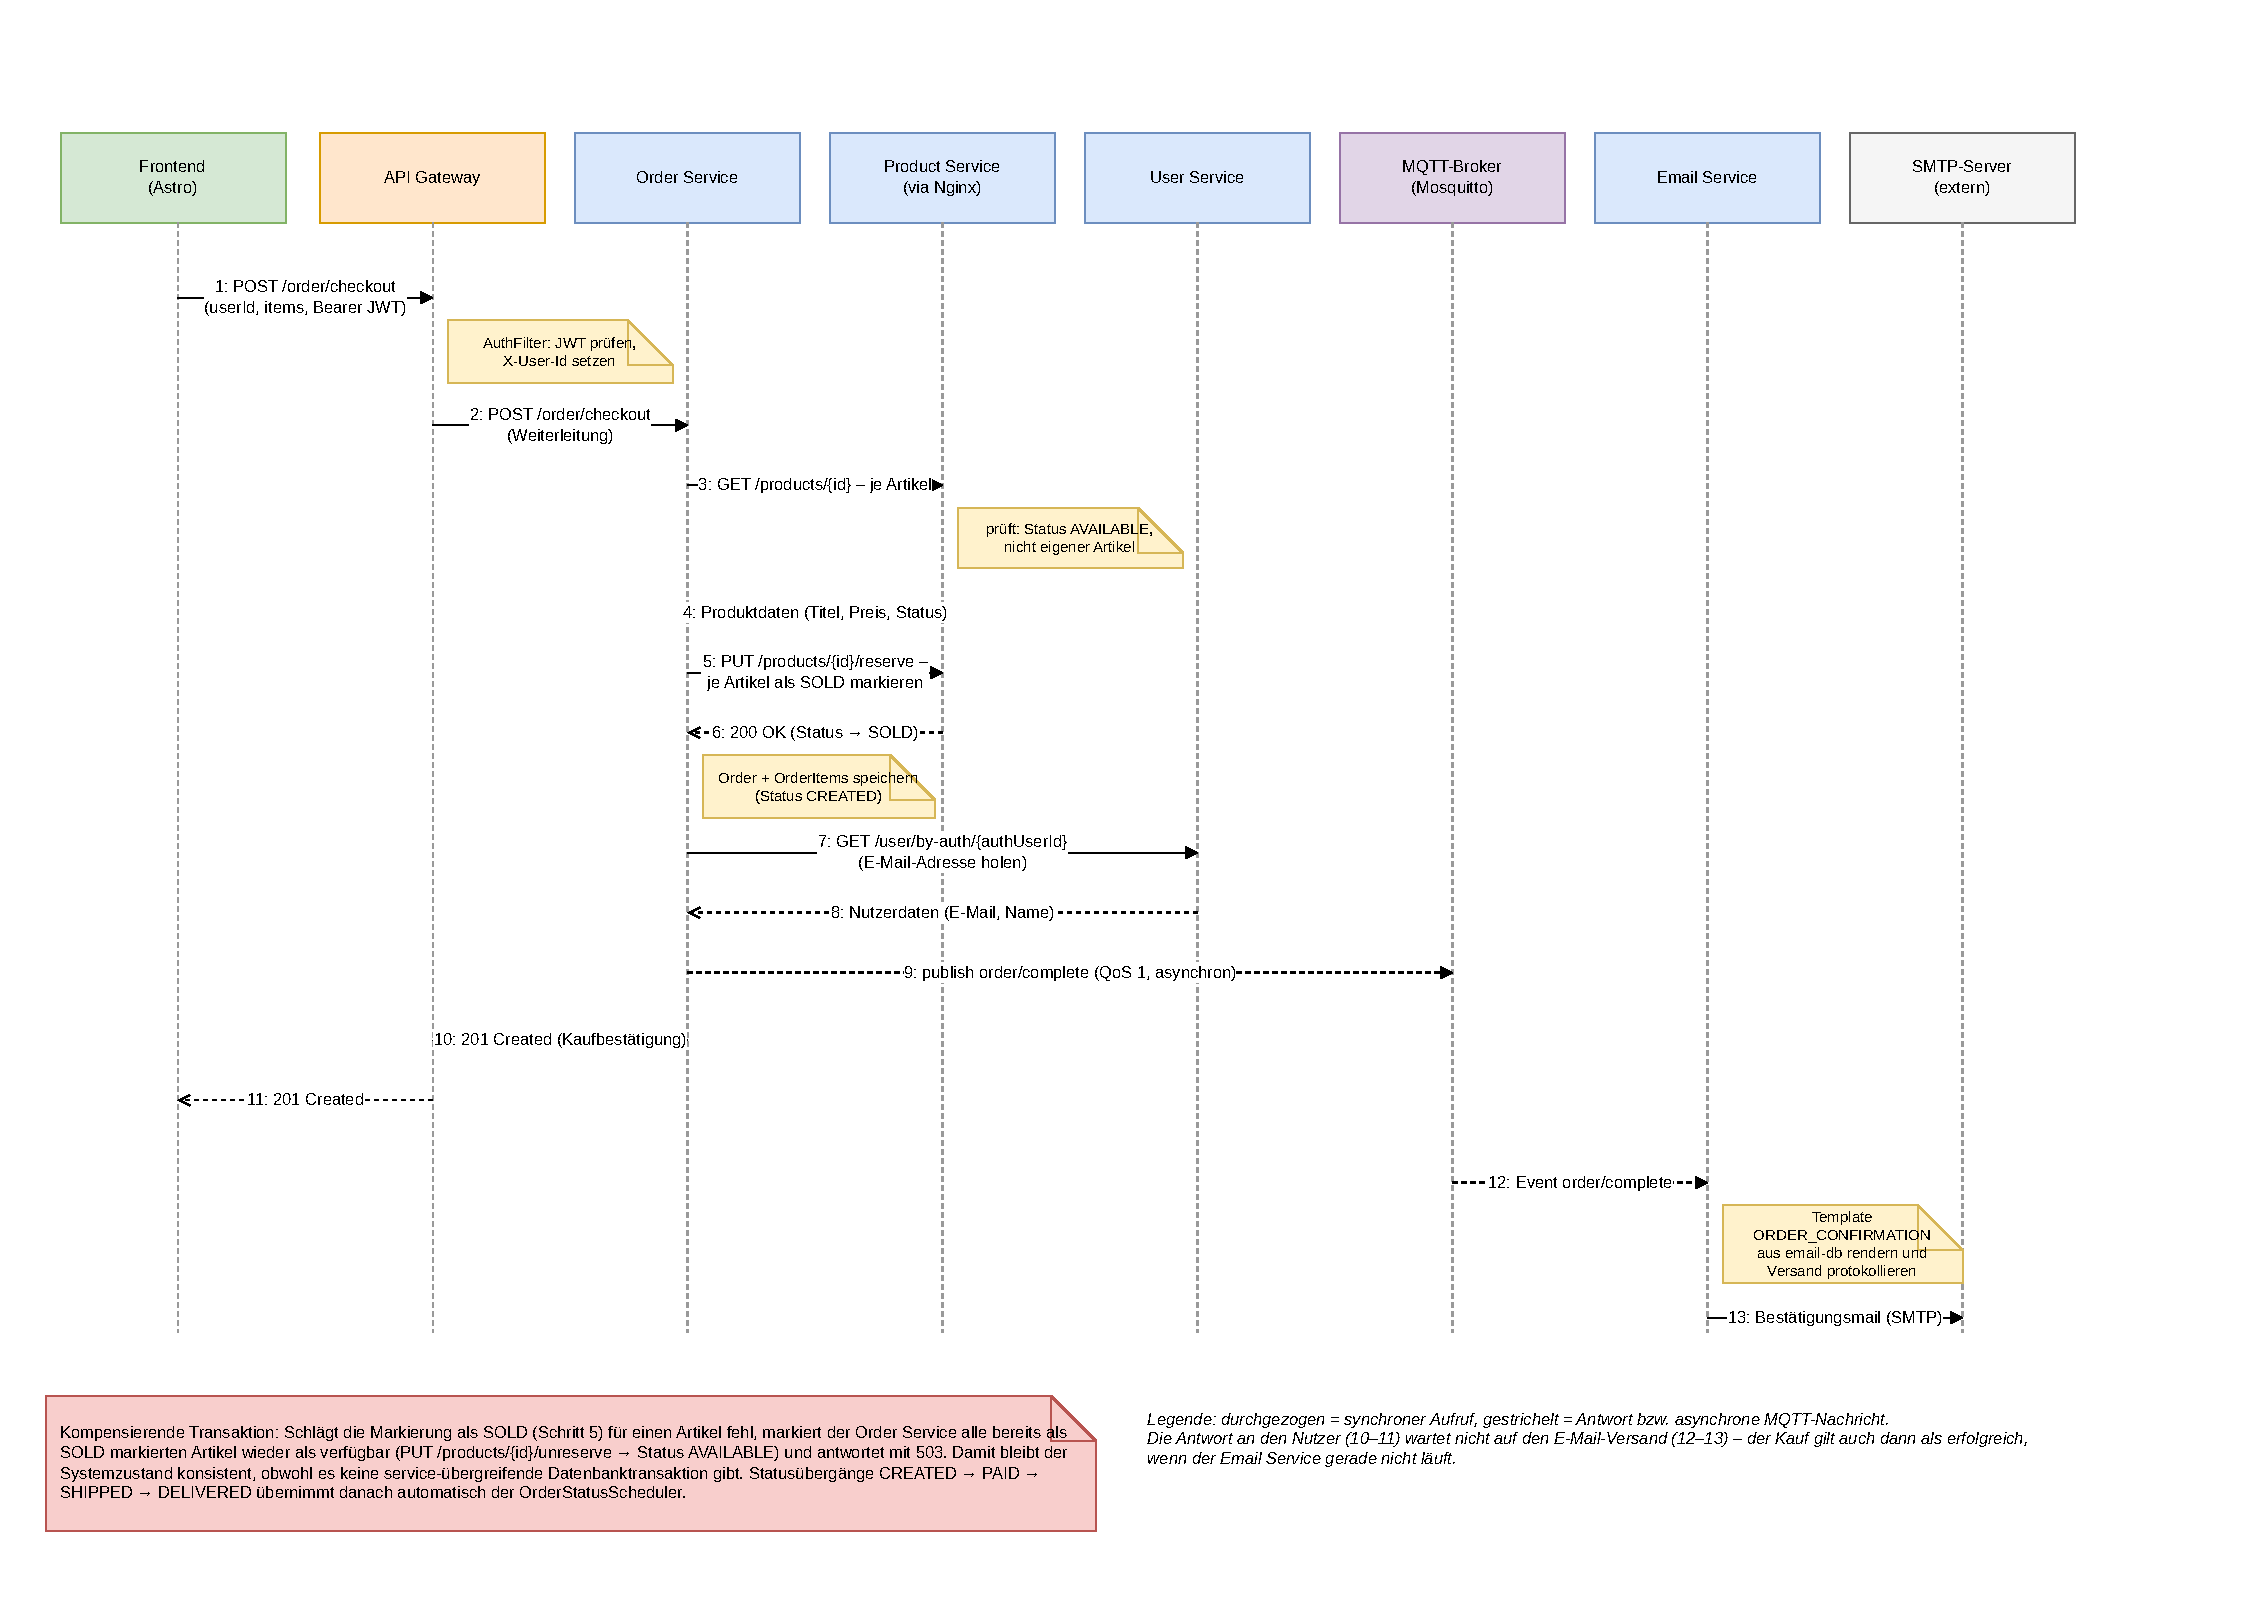
\includegraphics[width=\linewidth]{images/03-sequenz-checkout}
    \caption{Kauf von Artikeln und Versand der Bestellbestätigung}
    \label{fig:buying}
\end{figure}
\section{Verteilungssicht}

\subsection{Infrastruktur -- Ebene 1}

Das Gesamtsystem wird mit Docker Compose betrieben. Alle Container befinden
sich im gemeinsamen Docker-Netzwerk \texttt{app-net}.

Nur das Frontend veröffentlicht mit Port~\texttt{4321} einen Port auf dem
Docker-Host. Es leitet Backend-Anfragen intern über
\texttt{http://api-gateway:8080} an das API Gateway weiter.

Die Services, Datenbanken und der MQTT-Broker sind ausschließlich innerhalb
des Docker-Netzwerks erreichbar. Der Product Service wird mit drei Replikaten
ausgeführt, auf die ein interner Nginx-Loadbalancer die Anfragen verteilt.
    {
    \renewcommand{\arraystretch}{1.4}

    \begin{table}[H]
        \centering
        \begin{tabularx}{\linewidth}{
                >{\bfseries\raggedright\arraybackslash}p{0.25\linewidth}
                >{\raggedright\arraybackslash}p{0.14\linewidth}
                >{\raggedright\arraybackslash}p{0.18\linewidth}
                >{\raggedright\arraybackslash}X
        }
            \toprule
            \rowcolor{tableHeaderColor}
            Container & Host-Port & Interner Port & Anmerkung \\
            \midrule

            Frontend &
            4321 &
            4321 &
            Einziger von außen erreichbarer Container. \\

            \rowcolor{tableRowColor}
            API Gateway &
            -- &
            8080 &
            Zentraler Backend-Einstieg, nur intern erreichbar. \\

            Auth, User und Order Service &
            -- &
            8080 &
            Nur innerhalb von \texttt{app-net} erreichbar. \\

            \rowcolor{tableRowColor}
            Product Service &
            -- &
            8082 &
            Drei Replikate, nur intern erreichbar. \\

            Product-Service-Proxy &
            -- &
            80 &
            Interner Nginx-Loadbalancer. \\

            \rowcolor{tableRowColor}
            Email Service &
            -- &
            -- &
            Kommunikation ausschließlich über MQTT. \\

            MQTT-Broker &
            -- &
            1883, 9001 &
            Nur innerhalb von \texttt{app-net} erreichbar. \\

            \rowcolor{tableRowColor}
            PostgreSQL-Datenbanken &
            -- &
            5432 &
            Je zustandsbehaftetem Service eine Instanz. \\

            \bottomrule
        \end{tabularx}

        \caption{Container- und Portübersicht}
        \label{tab:container-ports}
    \end{table}
}
\begin{figure}[H]
  \centering
  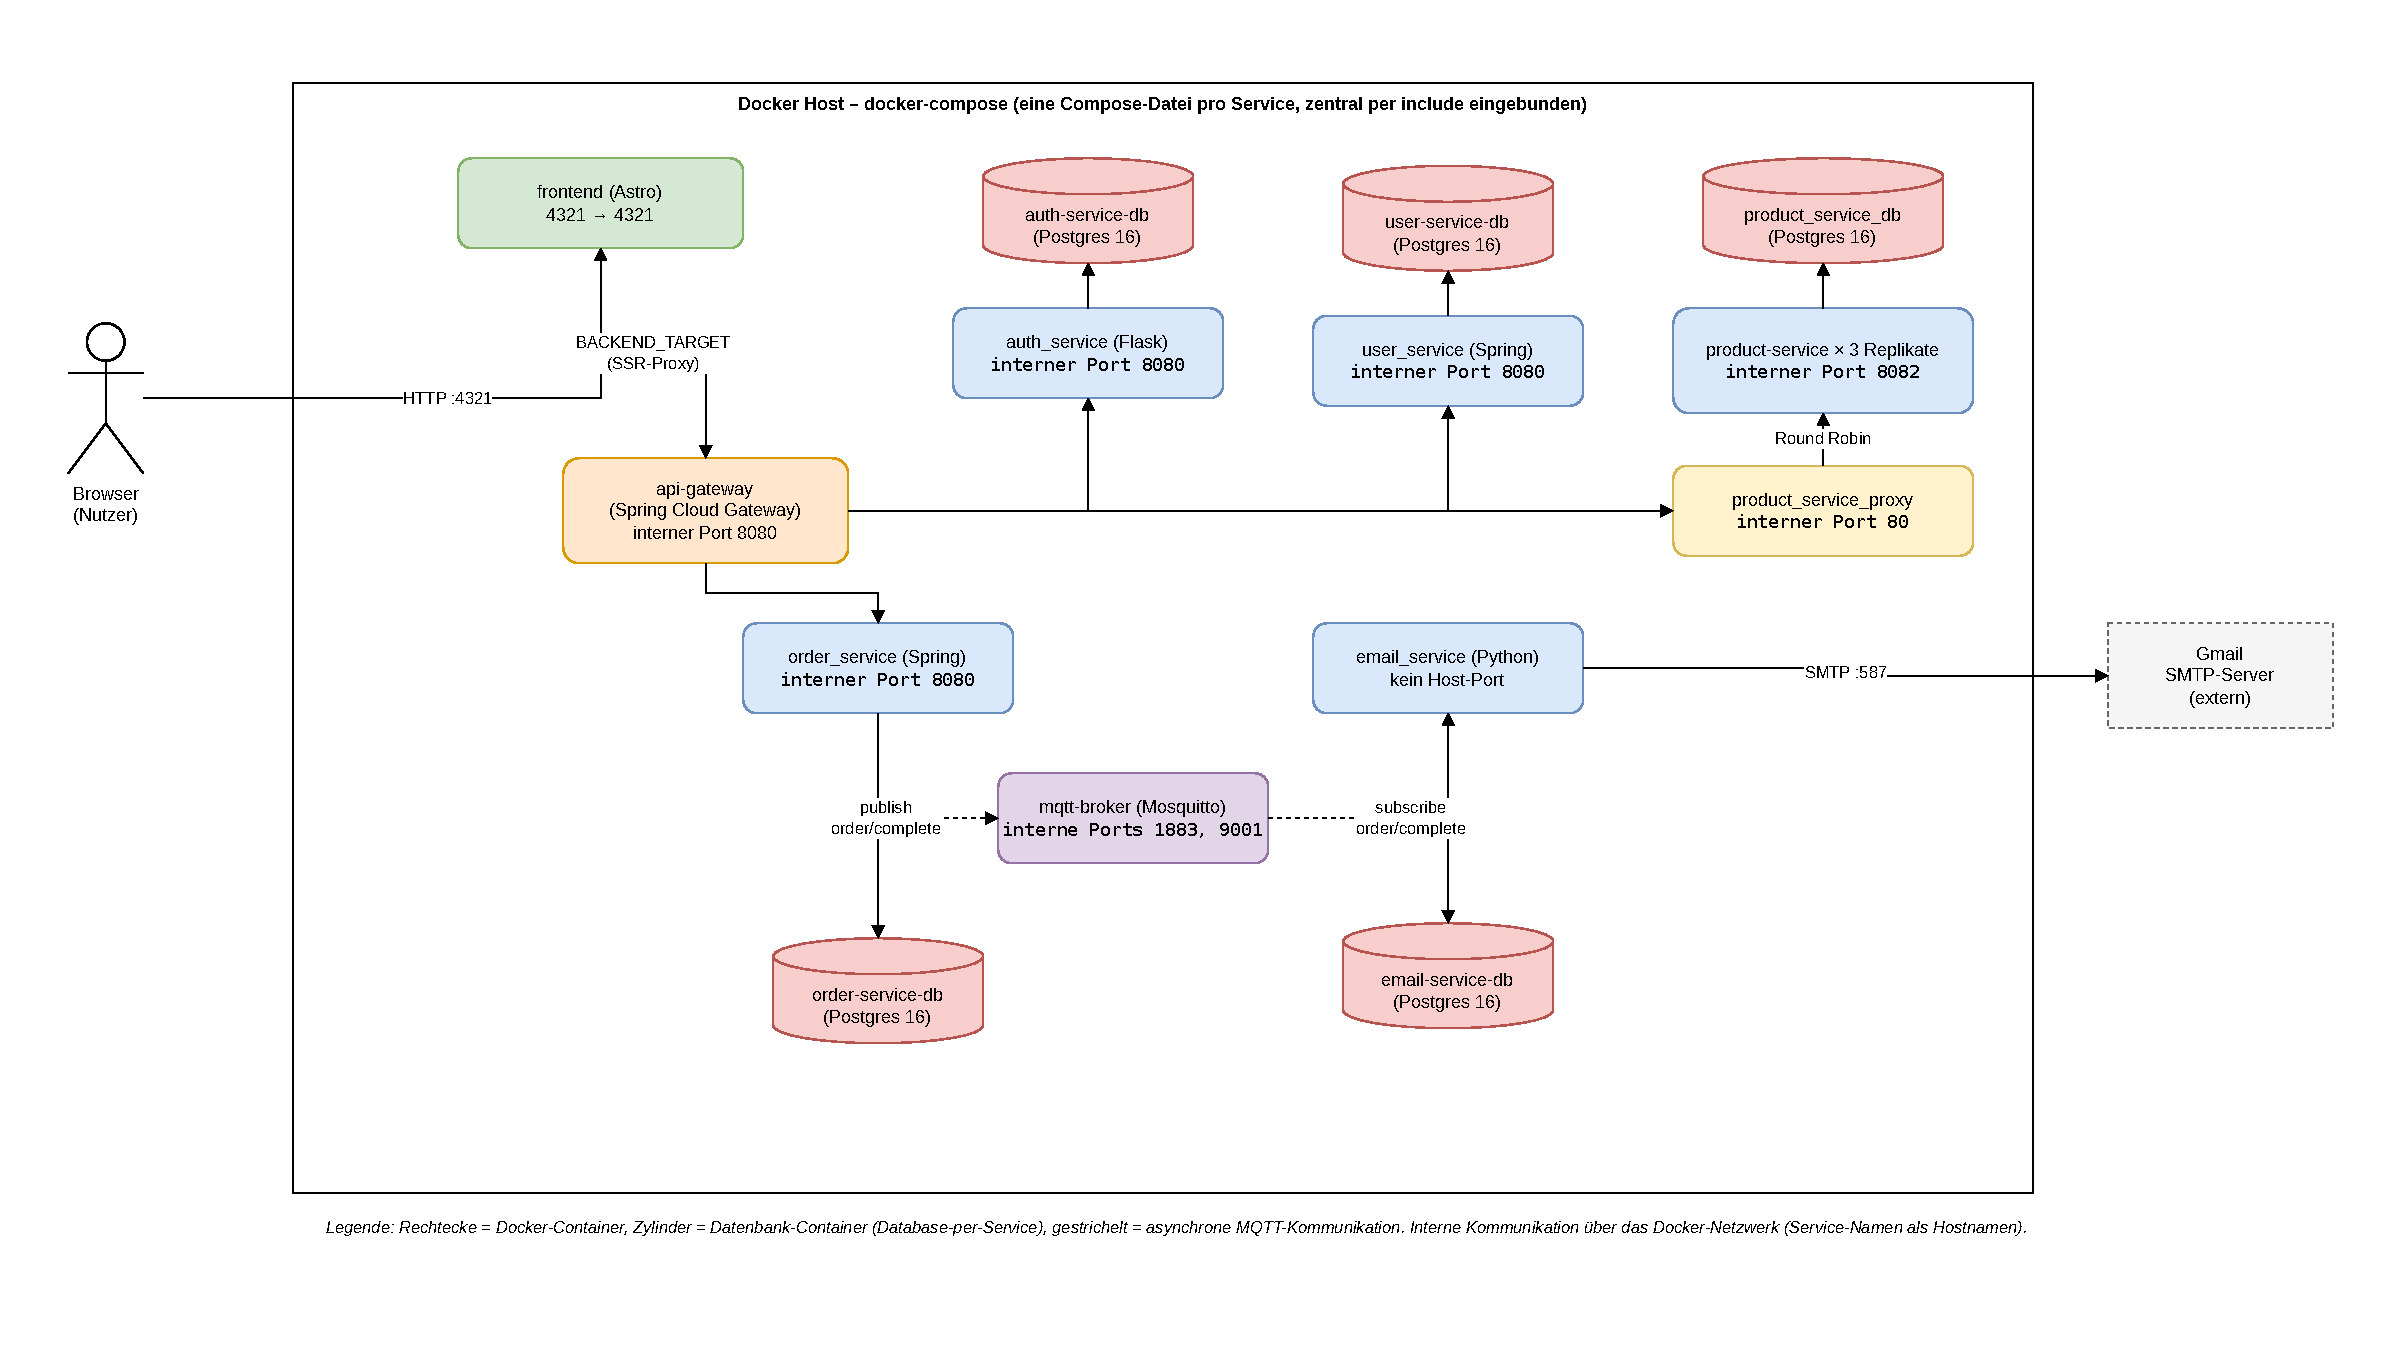
\includegraphics[width=\linewidth,trim=1cm 1.5cm 1cm 1cm,clip]{images/05-deployment}
  \caption{Deployment-Diagramm}
\end{figure}


\section{Querschnittliche Konzepte}

Die folgenden technischen Regeln gelten serviceübergreifend.

\subsection{Sicherheit}

Der Auth Service stellt JWTs mit einer Gültigkeit von 60 Minuten aus.
Das API Gateway validiert die Tokens und übergibt die Benutzer-ID über den Header \texttt{X-User-Id}.
Der interne Aufruf des User Service an den Auth Service wird zusätzlich durch den Header \texttt{X-Internal-Key} autorisiert.
\subsection{Kommunikation}

Synchrone Serviceaufrufe erfolgen über REST.
Bestellereignisse werden über MQTT mit Zustellbestätigung übertragen.

\subsection{Fehlerbehandlung}

Die Spring-basierten Services verwenden ein einheitliches Fehlerformat.
Validierungsfehler liefern \texttt{400}, fehlende Ressourcen \texttt{404}, Konflikte \texttt{409} und
unerwartete Fehler \texttt{500}.

\subsection{Datenhaltung}

Jeder zustandsbehaftete Service besitzt eine eigene PostgreSQL-Datenbank.
Nur der jeweilige Service darf direkt auf seine Datenbank zugreifen.
Serviceübergreifende Beziehungen werden über IDs statt über
datenbankübergreifende Fremdschlüssel abgebildet.

\subsection{Serviceübergreifende Konsistenz}

Serviceübergreifende Datenbanktransaktionen werden nicht verwendet.
Schlägt die Änderung eines Produkts während des Kaufvorgangs fehl, setzt der
Order Service bereits vorgenommene Änderungen durch kompensierende Aufrufe
zurück.

\subsection{Skalierung}

Die Instanzen des Product Service speichern keine Sitzungsdaten oder lokalen
Dateien. Dadurch können Anfragen über Nginx im Round-Robin-Verfahren auf drei
Replikate verteilt werden.

Alle Replikate greifen auf dieselbe \texttt{product-db} zu. Die Datenbank
kann daher bei hoher Last zum Engpass werden. Eine automatische,
lastabhängige Skalierung ist nicht umgesetzt; die Anzahl der Replikate wird
beim Start festgelegt.
\section{Architekturentscheidungen}

Die folgenden Entscheidungen prägen den Aufbau und die Implementierung
des Systems. Neben der Begründung werden auch die daraus entstehenden
Nachteile und zusätzlichen Aufwände betrachtet.

    {
    \renewcommand{\arraystretch}{1.4}

    \begin{tabularx}{\linewidth}{@{}
            >{\bfseries\raggedright\arraybackslash}p{0.09\linewidth}
            >{\raggedright\arraybackslash}p{0.22\linewidth}
            >{\raggedright\arraybackslash}X
            >{\raggedright\arraybackslash}X
        @{}}

\toprule
\rowcolor{tableHeaderColor}
Nr. & Entscheidung & Begründung & Konsequenz \\
\midrule

AE 1 &
Fachliche Aufteilung in eigenständige Services &
Authentifizierung, Benutzerverwaltung, Produkte, Bestellungen und
Benachrichtigungen besitzen getrennte Verantwortlichkeiten und sollen
unabhängig entwickelt werden können. &
Die Services können getrennt entwickelt und betrieben werden.
Dafür entstehen zusätzlicher Deployment-Aufwand, Netzwerkkommunikation
und verteilte Fehlerfälle. \\

\rowcolor{tableRowColor}
AE 2 &
Zentrales API Gateway &
Routing und JWT-Prüfung sollen nicht in jedem Service einzeln
implementiert werden. &
Das Gateway bildet einen einheitlichen Zugang, verursacht aber einen
zusätzlichen Netzwerkhop und ist ein zentraler Ausfallpunkt. \\

AE 3 &
Eigene Datenbank je Service &
Jeder Service soll alleiniger Eigentümer seiner Daten und seines
Datenmodells sein. &
Die Services bleiben hinsichtlich ihrer Datenhaltung unabhängig.
Serviceübergreifende Fremdschlüssel und gemeinsame Transaktionen sind
jedoch nicht möglich. \\

AE 4 &
Kompensation statt verteilter Transaktion &
Product Service und Order Service besitzen getrennte Datenbanken,
sodass keine gemeinsame Datenbanktransaktion verwendet werden kann. &
Bereits geänderte Produkte werden bei einem Fehler durch Gegenaufrufe
wieder freigegeben. Diese Rückabwicklung erfordert zusätzliche
Programmlogik. \\

\rowcolor{tableRowColor}
AE 5 &
Zustandslose Product-Service-Replikate &
Produktanfragen sollen exemplarisch auf mehrere Instanzen verteilt
werden können. &
Drei Product-Service-Instanzen können über Nginx angesprochen werden.
Die gemeinsam verwendete Produktdatenbank bleibt jedoch ein möglicher
Engpass. \\

\bottomrule
    \end{tabularx}
}
\section{Qualitätsanforderungen}

\subsection{Qualitätsszenarien}

Die Qualitätsziele aus Kapitel 1 werden anhand konkreter Szenarien
überprüft.

\begin{description}
    \item[Szenario 1 -- Ausfalltoleranz]
    Der Email Service ist nicht verfügbar. Bestellungen können weiterhin
    abgeschlossen werden, da der E-Mail-Versand über MQTT vom Kaufvorgang
    entkoppelt ist.

    \item[Szenario 2 -- Skalierbarkeit]
    Mehrere Produktanfragen treffen gleichzeitig ein. Nginx verteilt die
    Anfragen auf drei Instanzen des Product Service.

    \item[Szenario 3 -- Fehlerisolation]
    Der Order Service wird neu gestartet. Währenddessen bleiben Anmeldung
    und Produktkatalog weiterhin verfügbar.

    \item[Szenario 4 -- Erweiterbarkeit]
    Ein zusätzlicher Service kann über eine eigene Compose-Konfiguration und
    eine neue Route im API Gateway eingebunden werden, ohne bestehende
    Services grundlegend zu verändern.

    \item[Szenario 5 -- Sicherheit]
    Ein geschützter Endpunkt wird ohne gültiges JWT aufgerufen. Das API
    Gateway weist die Anfrage ab, bevor sie den Zielservice erreicht.
\end{description}
\section{Risiken und technische Schulden}

\begin{description}
  \item[Kein zentrales Logging/Monitoring]
    Es existiert keine Correlation-ID über Services hinweg; Fehlersuche
    im verteilten System ist erschwert.
  \item[Gateway als Single Point of Failure]
    Fällt das API Gateway aus, ist das gesamte System nicht
    erreichbar. Kein Failover-Mechanismus vorgesehen.
  \item[Zyklische Abhängigkeit]
    Product Service ↔ Order Service: Der Product Service ruft den
    Order Service beim Kauf auf, der Order Service ruft den Product
    Service für Produktdetails ab.
  \item[Secrets im Klartext]
    JWT-Secret und SMTP-Zugangsdaten liegen unverschlüsselt in den
    Docker-Compose-Dateien.
  \item[ID-Typ-Inkonsistenz]
    \texttt{auth\_service} und \texttt{user\_service} verwenden UUIDs,
    \texttt{product\_service} und \texttt{order\_service} wurden auf
    Long umgestellt. Die \texttt{X-User-Id}-Kette ist damit
    aktuell nicht durchgängig funktionsfähig.
\end{description}

\section{Fazit}

Die Umsetzung verdeutlicht sowohl die Vorteile als auch die Nachteile einer Microservice-Architektur.
Die fachliche Aufteilung, klar definierte Schnittstellen und
getrennte Datenbanken ermöglichen eine weitgehend unabhängige Entwicklung der einzelnen Services.
Durch die Kombination aus synchroner und asynchroner Kommunikation konnten unterschiedliche Formen der Servicekopplung praktisch umgesetzt und erprobt werden.

Gleichzeitig erhöht die Verteilung der Anwendung den technischen Aufwand.
Betrieb und Fehlersuche erstrecken sich über mehrere Services, Container und Kommunikationswege.
Serviceübergreifende Vorgänge können nicht durch eine gemeinsame Datenbanktransaktion abgesichert werden und
benötigen deshalb zusätzliche Kompensationslogik.
Zudem bleibt der Kaufvorgang von synchron aufgerufenen Services wie dem Product Service und dem User Service abhängig.

Für größere Systeme mit mehreren Entwicklungsteams,
unterschiedlich belasteten Teilbereichen oder
hohen Anforderungen an die Fehlerisolation kann eine Microservice-Architektur sinnvoll sein.
Für den begrenzten Umfang der umgesetzten Beispielanwendung wäre ein modularer Monolith einfacher zu entwickeln und
zu betreiben gewesen.
Als Lernprojekt war die gewählte Architektur dennoch geeignet, da ihre Auswirkungen auf Implementierung,
Kommunikation, Datenhaltung und Fehlerbehandlung praktisch untersucht werden konnten.
\section{Dokumentation der Verwendung von KI-Werkzeugen}

\begin{table}[H]
    \centering
    {
        \renewcommand{\arraystretch}{1.5}
        \rowcolors{2}{tableRowColor}{white}
        \begin{tabularx}{\linewidth}{
                >{\bfseries\raggedright\arraybackslash}p{0.33\linewidth}
                >{\raggedright\arraybackslash}X
                >{\raggedright\arraybackslash}p{0.33\linewidth}
        }
        \toprule
        \rowcolor{tableHeaderColor}
        Zweck der Verwendung & Eingesetztes KI-Werkzeug & Verwendungsweise bzw. -ort \\
        \midrule

        Überarbeitung von Formulierungen und Schreibstil &
        ChatGPT GPT-5.6 SOL &
        Punktuelle Vorschläge für alternative Formulierungen sowie sprachliche und stilistische Überarbeitungen einzelner Textabschnitte \\

        Unterstützung bei der Entwicklung mit Java und Spring Boot &
        Claude Code,

        ChatGPT GPT-5.6 SOL,

        DeepSeek V4 Flash Free &
        Punktuelle Unterstützung bei der Fehlersuche, der Überprüfung bestehender Implementierungen und der Ausarbeitung einzelner Codevorschläge für die Java-Spring-Boot-Services \\

        Unterstützung bei der Entwicklung mit Python &
        ChatGPT GPT-5.6 SOL,

        DeepSeek V4 Flash Free &
        Punktuelle Unterstützung bei der Fehlersuche, der Anpassung bestehender Implementierungen und der Ausarbeitung einzelner Codevorschläge für die Python-Komponenten \\

        Unterstützung bei der Frontend-Entwicklung mit Astro und SolidJS &
        Claude Code &
        Punktuelle Unterstützung bei der Fehlersuche, der Überprüfung bestehender Komponenten und der Ausarbeitung einzelner Lösungsvorschläge für Astro, SolidJS, JavaScript, HTML und CSS \\

        \bottomrule
        \end{tabularx}}

    \caption{KI-Werkzeugen}
\end{table}



\end{document}
